\documentclass{report}
\usepackage{graphicx}
\usepackage{xcolor}
\usepackage[a4paper, total={6in, 8in}]{geometry}
\graphicspath{ {./image/} }

\title{Babar Forecasting}
\date{2020} 
 
\begin{document} 
\maketitle

\chapter{Goal}


\chapter{Data Management}

\section{Selection and Gathering}

There are too many products to have a prediction for each one. So we decided to gather them into categories. We want to gather them into pertinent groups so that the forecast can really help the bar. 

\subsection{First Selection}

The first step is to choose which product we are going to take account of. We choosed to focus our work on the drinks sales that had at least been sold ???. So we exclude any food or other kind of sales. 

SQL Request too extract those product : \\
 \\

CREATE TABLE WantedProducts AS
    SELECT babar$\_$server$\_$purchase.* FROM babar$\_$server$\_$purchase JOIN babar$\_$server$\_$product ON product$\_$id = babar$\_$server$\_$product.id WHERE NAME = 'Leffe' OR NAME = 'Hoegaaden blanche' OR NAME = 'Desperados' OR NAME = 'Smirnoff' OR NAME = 'Pastis' OR NAME = 'Hard' OR NAME = 'Grimbergen' OR NAME = 'Chimay Rouge' OR NAME = 'Chimay Bleue' OR NAME = 'Kro Demi' OR NAME = 'Cidre Demi' OR NAME = 'Pelforth' OR NAME = 'Kwak' OR NAME = 'Kir' OR NAME = 'Kro Pinte' OR NAME = 'Cidre Pinte' OR NAME = 'Cocktail Hard' OR NAME = 'Chimay Blanche' OR NAME = 'Shot'  OR NAME = 'Blanche Demi' OR NAME = 'Blanche Pinte' OR NAME = 'Cidre Doux/Brut' OR NAME = 'Ambree demi' OR NAME = 'Ambree Pinte'  OR NAME = 'Delirium' OR NAME = 'Rouge Pinte' OR NAME = 'Sangria' OR NAME = 'Karmeliet Triple' OR NAME = 'Duvel' OR NAME = 'Granita Hard' OR NAME = 'Skoll' OR NAME = 'Rouge Demi' OR NAME = '$1664$ Blanche' OR NAME = 'Chimay bleue' OR NAME = 'Pecheresse' OR NAME ='Cuvee des Trolls'  OR NAME = 'Kriek' OR NAME = 'Elephant Pinte' OR NAME = 'Elephant Demi' OR NAME = 'Maredsous Triple' OR NAME = 'Hard Qualite' OR NAME = 'BrewDog Punk IPA' OR NAME = 'JagerBomb' OR NAME = 'Cubanisto' OR NAME = 'Chouffe Pinte' OR NAME = 'Chouffe Demi' OR NAME = 'Corona' OR NAME = 'Tigre Bock' OR NAME = 'Troll Pinte' OR NAME = 'Troll Demi' OR NAME = 'Triple Karmeliet Pinte' OR NAME = 'Triple Karmeliet Demi' OR NAME = 'Paix Dieu $33$cL' OR NAME = 'Grim Triple Demi' OR NAME = 'Grim Triple Pinte' OR NAME = 'Cherry chouffe' OR NAME = 'Delirium rouge pinte' OR NAME = 'bush ambree' OR NAME = 'San Miguel';
		
List of considered product :

So now we have a data table gathering only the product we choose.

\subsection{Other products that could be considered}

\subsection{Regrouping them into categories}

A majority of this product has been coming and leaving from the bar menu so their sales aren't usable one by one. Therefor we decided to group them into pertinent categories. But how to choose this categories ? Here are our first thought.


High Degree Beers 
\begin{itemize}
\item Chimay Bleu
\item Kwak
\item Karmeliet Triple 
\item Duvel
\item Chimay bleue
\item Maredsous Triple
\item Chouffe Pinte
\item Chouffe Demi
\item Triple Karmeliet Pinte
\item Triple Karmeliet Demi
\item Grim Triple Pinte
\item Grim Triple Demi
\item bush ambree
\item Delirium
\item Elephant Pinte
\item Elephant Demi
\end{itemize}

Normal Degree Beers 
\begin{itemize}
\item Leffe
\item Grimbergen
\item Kro Demi
\item Kro Pinte
\item Pelforth
\item Skoll
\item BrewDog Punk IPA
\item Tigre Bock
\item Troll Pinte
\item Troll Demi
\item Cuvée des trolls
\item Paix Dieu 33cL
\item San Miguel
\item Ambrée Pinte
\item Ambrée Demi
\end{itemize}

Not Beer
\begin{itemize}
\item Smirnoff
\item Pastis
\item Hard
\item Kir
\item Cocktail Hard
\item Shot
\item Rouge Pinte 
\item Rouge Demi
\item Sangria
\item Granita Hard
\item Hard Qualite
\item JagerBomb
\end{itemize}

Special Beers 
\begin{itemize}
\item Desperados
\item Cidre Demi
\item Cidre Pinte
\item Cidre Doux/Brut
\item Cubanisto
\item Corona
\end{itemize}

Aromatized Beer
\begin{itemize}
\item Chimay Rouge
\item Hoegaaden blance
\item Chimay Blanche
\item Blanche Demi
\item Blanche Pinte
\item 1664 Blanche
\item Pecheresse
\item Kriek
\item Cherry chouffe
\item Delirium rouge pinte
\end{itemize}

Other idea : Aromatize beer and Special together

Those are ideas of the categories, at every time at least one product of each category was being sold, assuring the continuity of sales in each categories. The goal is having sales that are homogene on a year scale.

\section{Time Scale}

We think that a Weekly prediction can be done, so we'll consider the sales week by week (Time series approach). If we have difficulties doing it we will consider doing it monthly but then the forecast would be much less usable. (Time series approach)

We will also maybe consider a year index. Indeed promotion aren't all the sames therefor they don't consume the same quantities. Adding a bias for each promotion (which would be compute thanks to the first month of data ? september ?) could maybe increase the accuracy of our estimations.
\subsection{Sorting By week}

I don't think that I can sort the data by week by using SQL, so I'll do a python code that do that. The results will be a table with the sales for each category for each week.


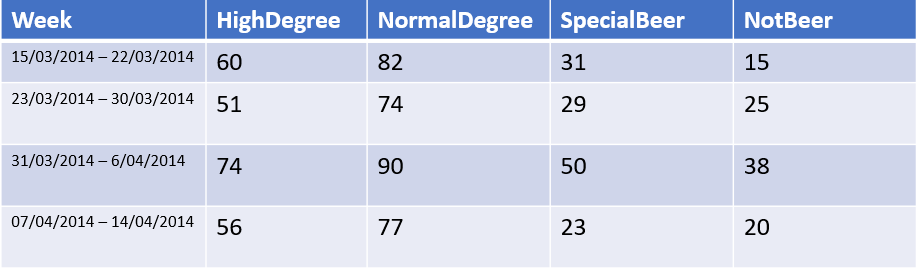
\includegraphics{FormatTable}

\section{Given Data}

In order to do our prediction we thing about using the following features :
\begin{itemize}
\item Day before next holiday 
\item Day before next exam
\item Day after exam or holiday ?
\item Day before next large event ?
\item Date of each sale
\end{itemize}

We think that those are the main influences on whether people buy more or less drinks in a bar.


\section{}

\chapter{Machine Learning Methods}

Now the core of our work is to choose the best method to predict from our data. Or goal is to look in the dataset for features such as trends, cyclical fluctuations, seasonality, and behavioral patterns.



Here are the algorithm that we read about and could be used to forecast sales :
\begin{itemize}
\item
\item
\item
\end{itemize}

\chapter{Development Ideas}



\chapter{Inspirations}

https://towardsdatascience.com/sales-forecasting-from-time-series-to-deep-learning-5d115514bfac : Forecasting principles and basis 

https://medium.com/analytics-vidhya/walmart-sales-forecasting-d6bd537e4904 : Forecasting at Walmart 





\end{document}